\documentclass[conference]{IEEEtran}
\IEEEoverridecommandlockouts
\usepackage{cite}
\usepackage{amsmath,amssymb}
\usepackage{graphicx}
\usepackage{booktabs}
\usepackage{multirow}
\usepackage{algorithm}
\usepackage{algpseudocode}
\usepackage{xcolor}
\usepackage{tikz}
\usetikzlibrary{arrows.meta,positioning,calc}
\usepackage{pgfplots}
\usepgfplotslibrary{groupplots}
\pgfplotsset{compat=1.17}
\usepackage[hidelinks]{hyperref}

% Colour-blind-safe palette (Okabe--Ito) for setups and flows
\definecolor{cBE}{HTML}{999999}
\definecolor{cMO}{HTML}{E69F00}
\definecolor{cML}{HTML}{56B4E9}
\definecolor{cST}{HTML}{009E73}
\definecolor{cOR}{HTML}{0072B2}
\definecolor{cUR}{HTML}{0072B2}
\definecolor{cPL}{HTML}{D55E00}
\definecolor{cMM}{HTML}{E69F00}

\begin{document}

\title{Capacity-Aware SDN Orchestration of V2X Network Slices with Metering, Strict Priority and Mobility Handling on an Emulated Vehicular Edge Testbed}

\author{\IEEEauthorblockN{A. Adharsh, Rishabh Bhat, Samuel Gerald and Navin Kumar}
\IEEEauthorblockA{Department of Electronics and Communication Engineering, Amrita School of Engineering, Bengaluru\\
Amrita Vishwa Vidyapeetham, India\\
Email: \{bl.en.u4ece23101, bl.en.u4ece23240, bl.en.u4ece23245\}@bl.students.amrita.edu}}

\maketitle

\begin{abstract}
Vehicles share roadside infrastructure among traffic classes with very different needs, and safety messages suffer once bulk infotainment saturates the backhaul. This paper presents an orchestrator, written as a RYU application over OpenFlow~1.3, that maps vehicle-to-everything (V2X) traffic onto five slices, polices each slice with a switch meter, tags packets with DSCP for strict-priority backhaul queues, tracks vehicles across roadside-unit handovers, and every 2\,s resizes the broadband slice to the capacity left by critical traffic. We evaluate it on a Mininet-WiFi testbed with six vehicles, two roadside units and edge servers, using an ablation of five configurations over four scenarios with five repetitions (80 trials). Under a broadband flood, the 95th-percentile platoon delay falls from 3.8\,s to 24.9\,ms with no loss. Under heavy critical load, metering alone gives 203\,ms, whereas the orchestrator holds 23.2\,ms. The open, scripted testbed lets researchers and operators prototype and compare vehicular slicing policies on a single machine.
\end{abstract}

\begin{IEEEkeywords}
V2X, network slicing, software-defined networking, OpenFlow meters, strict-priority scheduling, Mininet-WiFi, edge computing
\end{IEEEkeywords}

% =====================================================================
\section{Introduction}

Connected and automated driving depends on a steady exchange of messages between vehicles, roadside units (RSUs) and servers. These services ask very different things of the network. Cooperative awareness and emergency warnings are small and periodic, yet they must arrive within tens of milliseconds with high reliability; platooning and sensor sharing tighten these bounds further~\cite{3gpp22186}. In the same cell, passengers stream video and download maps, which demands throughput but tolerates delay. The New Radio sidelink and its cellular counterpart give vehicles the radio means to carry both kinds of traffic~\cite{garcia2021tutorial}. However, the RSU uplinks and the aggregation links behind them are shared and of finite capacity, so traffic of one kind can still delay traffic of another.

Network slicing answers this by carving one physical infrastructure into logical networks, each with its own resources and service guarantees~\cite{foukas2017slicing}. Its practical form depends on softwarization: the control logic is moved out of individual devices into programmable functions that can be reconfigured at run time~\cite{afolabi2018slicing}. Software-defined networking (SDN) supplies the needed mechanism. With OpenFlow, a logically centralized controller installs match--action rules in switches, reads their counters, and changes their behaviour without touching hardware~\cite{mckeown2008openflow}, and the approach has matured into a broad ecosystem of controllers and data planes~\cite{kreutz2015sdn}. Applied to vehicular networks, slicing lets an operator give safety, cooperative-driving, infotainment and telemetry traffic separate treatment over the same roadside equipment~\cite{campolo2017v2x}.

Several studies have brought these ideas into vehicular settings. Early software-defined VANET designs showed that a central controller can steer vehicular flows and adapt routes~\cite{ku2014sdvanet}. Campolo \emph{et al.} used OpenFlow metering over an emulated wireless network to keep automotive slices apart~\cite{campolo2018road}, and Saraiva \emph{et al.} built an application-driven framework that combines a RYU controller, an emulated access network and a road simulator, and compared it with best-effort and QoS-only operation~\cite{saraiva2021its}. These works rely on emulators such as Mininet-WiFi, which runs real network stacks with a wireless channel model on one host~\cite{fontes2015mininetwifi}. Three gaps remain. First, slice budgets are usually fixed, or are changed on coarse triggers that ignore how much capacity the shared link actually has left. Second, rate policing and packet scheduling are rarely evaluated together, so it is unclear when policing alone is enough. Third, practical pitfalls of Wi-Fi roadside units, such as stale station entries after a handover and traffic bridged inside the access point, are seldom reported, although they silently break slice isolation.

This paper addresses these gaps. Its original contributions and novelty are:
\begin{itemize}
\item \textbf{A closed-loop, capacity-aware reallocation policy} that reads OpenFlow meter counters every 2\,s and sets the broadband slice to the capacity the critical slices leave on the backhaul, with step quantization, a floor, and explicit protect/adjust/release states.
\item \textbf{Joint enforcement by meters and strict priority}: per-slice meters for isolation, plus controller-written DSCP marks that drive a three-band strict-priority queue on both ends of every backhaul link, without disturbing the emulated link rate and delay.
\item \textbf{Mobility-aware forwarding for Wi-Fi RSUs} that detects handovers from port changes and flushes stale rules network-wide, and two fixes that keep slicing intact across mobility: fast station expiry with vehicle beacons, and client isolation with hairpin forwarding so that same-RSU traffic cannot bypass its meter.
\item \textbf{A reproducible ablation benchmark}: five configurations that add one mechanism at a time, four scenarios including scripted handover and random-waypoint mobility, five repetitions each (80 trials), with per-packet latency, jitter, loss and outage metrics, all released with the testbed scripts and a replay dashboard.
\end{itemize}

The remainder of the paper is organized as follows. Section~II describes the system architecture. Section~III details the design of the slices, the enforcement mechanisms, the reallocation loop, the mobility handling and the measurement method. Section~IV presents and discusses the results, and Section~V concludes with the challenges faced and directions for future work.

% =====================================================================
\section{System Architecture}

Fig.~\ref{fig:arch} shows the testbed. The data plane consists of three Open vSwitch instances controlled over OpenFlow~1.3. Two of them, \emph{rsu1} and \emph{rsu2}, are IEEE~802.11g access points on channels 1 and 6 with a 30\,m range, and each has a multi-access edge computing (MEC) server attached by a 0.5\,ms link. The third, \emph{s1}, aggregates the two RSUs over backhaul links of 20\,Mb/s and 5\,ms each, and connects a central infotainment server and a telemetry server over a 100\,Mb/s, 15\,ms link. The backhaul is deliberately the bottleneck of the network. Six vehicles are Wi-Fi stations; they either follow scripted, intersecting paths that force handovers between the RSUs, or move under a seeded random-waypoint model at 2--4\,m/s. The whole network runs in Mininet-WiFi with the wmediumd channel model~\cite{fontes2015mininetwifi}, so association, signal loss and re-association are emulated rather than assumed.

\begin{figure*}[t]
\centering
\resizebox{0.96\textwidth}{!}{% Fig. 1: testbed topology and orchestrator modules (drawn in TikZ)
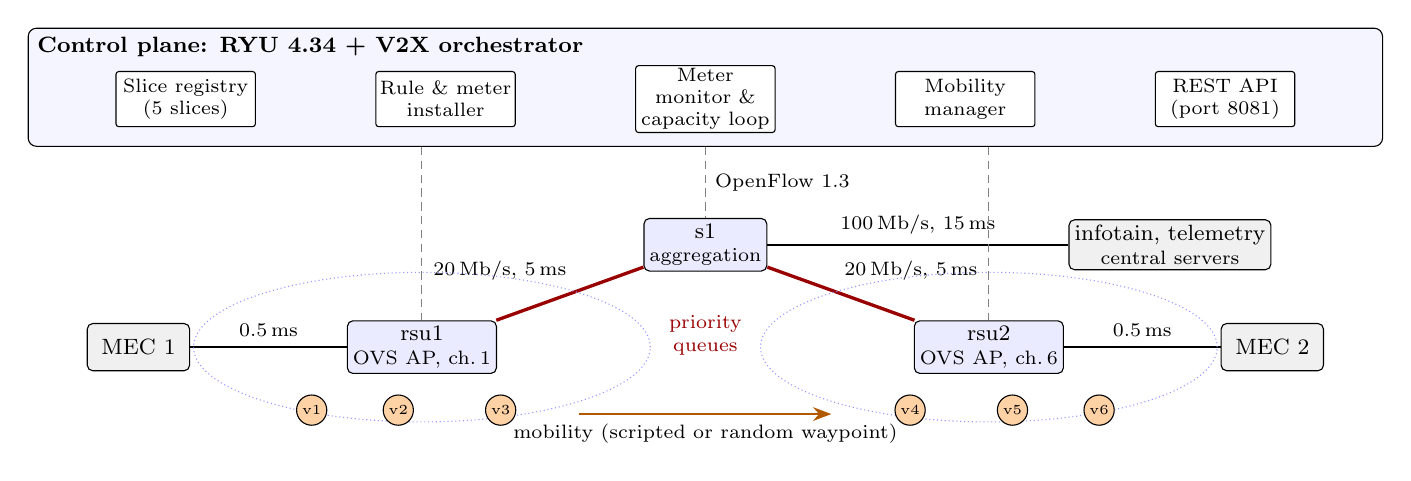
\begin{tikzpicture}[font=\footnotesize, >=Stealth,
  box/.style={draw, rounded corners=2pt, align=center, minimum height=6mm, inner sep=2pt},
  sw/.style={box, fill=blue!8, minimum width=15mm},
  srv/.style={box, fill=gray!12, minimum width=13mm},
  mod/.style={draw, fill=white, rounded corners=1pt, align=center, font=\scriptsize, minimum height=7mm, text width=17mm, inner sep=1pt},
  veh/.style={draw, circle, fill=orange!35, inner sep=1.2pt, font=\tiny},
  bh/.style={very thick, red!60!black},
  ctl/.style={densely dashed, gray}]
  % controller
  \node[draw, rounded corners=3pt, fill=blue!4, minimum width=172mm, minimum height=15mm] (ctrl) at (0,4.1) {};
  \node[anchor=north west, font=\footnotesize\bfseries] at (ctrl.north west) {Control plane: RYU 4.34 + V2X orchestrator};
  \node[mod] (m1) at (-6.6,3.95) {Slice registry\\(5 slices)};
  \node[mod] (m2) at (-3.3,3.95) {Rule \& meter\\installer};
  \node[mod] (m3) at (0,3.95) {Meter monitor \&\\capacity loop};
  \node[mod] (m4) at (3.3,3.95) {Mobility\\manager};
  \node[mod] (m5) at (6.6,3.95) {REST API\\(port 8081)};
  % data plane
  \node[sw] (s1) at (0,2.1) {s1\\[-1pt]\scriptsize aggregation};
  \node[sw] (r1) at (-3.6,0.8) {rsu1\\[-1pt]\scriptsize OVS AP, ch.\,1};
  \node[sw] (r2) at (3.6,0.8) {rsu2\\[-1pt]\scriptsize OVS AP, ch.\,6};
  \node[srv] (cs) at (5.9,2.1) {infotain, telemetry\\[-1pt]\scriptsize central servers};
  \node[srv] (e1) at (-7.2,0.8) {MEC 1};
  \node[srv] (e2) at (7.2,0.8) {MEC 2};
  \draw[bh] (s1) -- node[above left, font=\scriptsize, text=black, pos=0.45] {20\,Mb/s, 5\,ms} (r1);
  \draw[bh] (s1) -- node[above right, font=\scriptsize, text=black, pos=0.45] {20\,Mb/s, 5\,ms} (r2);
  \draw[thick] (s1) -- node[above, font=\scriptsize] {100\,Mb/s, 15\,ms} (cs);
  \draw[thick] (r1) -- node[above, font=\scriptsize] {0.5\,ms} (e1);
  \draw[thick] (r2) -- node[above, font=\scriptsize] {0.5\,ms} (e2);
  \draw[ctl] (ctrl.south) -- node[right, font=\scriptsize, text=black] {OpenFlow 1.3} (s1);
  \draw[ctl] (ctrl.south -| r1) -- (r1);
  \draw[ctl] (ctrl.south -| r2) -- (r2);
  % coverage and vehicles
  \draw[blue!40, densely dotted] (r1) ellipse (2.9 and 0.95);
  \draw[blue!40, densely dotted] (r2) ellipse (2.9 and 0.95);
  \foreach \x/\n in {-5.0/1,-3.9/2,-2.6/3,2.6/4,3.9/5,5.0/6} {\node[veh] at (\x,0.0) {v\n};}
  \draw[->, orange!70!black, thick] (-1.6,-0.05) -- node[below, font=\scriptsize, text=black] {mobility (scripted or random waypoint)} (1.6,-0.05);
  \node[font=\scriptsize, text=red!60!black, align=center] at (0,0.95) {priority\\queues};
\end{tikzpicture}
}
\caption{Testbed architecture. The orchestrator runs as a RYU application and controls both RSUs and the aggregation switch \emph{s1}; strict-priority queues sit on both ends of each 20\,Mb/s backhaul link.}
\label{fig:arch}
\end{figure*}

The control plane is a RYU~4.34 controller hosting the orchestrator, which is organized in five modules (Fig.~\ref{fig:arch}). The \emph{slice registry} holds each slice's traffic signature, meter identifier, budget and DSCP value. The \emph{rule and meter installer} programs every switch as soon as it connects. The \emph{meter monitor} polls meter statistics and runs the reallocation loop. The \emph{mobility manager} learns where each vehicle is and reacts to handovers. A northbound \emph{REST interface} on port 8081 lists slices and events and lets an operator resize any slice at run time.

Fig.~\ref{fig:pipeline} traces a packet through a switch. Table~0 classifies it by transport protocol and port, in both directions so that replies are classified too; the matching rule sends it through the slice meter, writes the slice's DSCP code point, and passes it to table~1, which forwards it on the learned port. On a backhaul port, the packet then enters a Linux queueing tree: a hierarchical token bucket (HTB) shaper at the link rate, a three-band strict-priority scheduler that reads the DSCP field, and a 5\,ms delay stage per band. Placing priority under the shaper keeps the emulated link rate and delay unchanged while deciding which packet leaves first.

\begin{figure}[t]
\centering
\resizebox{\columnwidth}{!}{% Fig. 2: per-switch packet pipeline, backhaul queue discipline and the reallocation loop (drawn in TikZ)
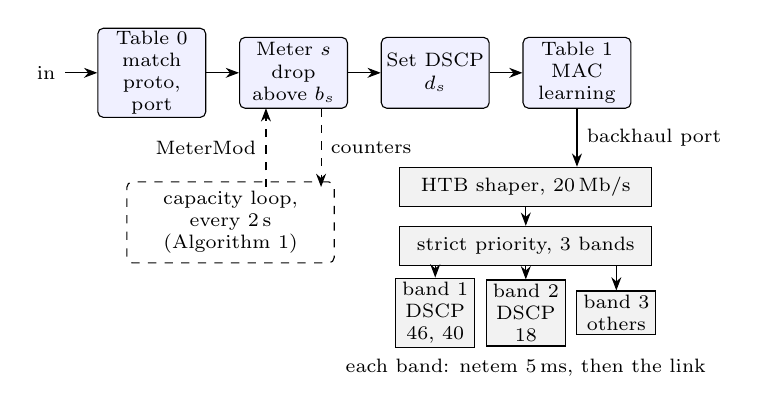
\begin{tikzpicture}[font=\scriptsize, >=Stealth,
  st/.style={draw, rounded corners=2pt, fill=blue!6, align=center, minimum height=9mm, text width=13mm, inner sep=1pt},
  q/.style={draw, fill=gray!10, align=center, minimum height=5mm, inner sep=1.5pt}]
  % pipeline
  \node[st] (t0) at (0,0) {Table 0\\match proto, port};
  \node[st] (m)  at (1.8,0) {Meter $s$\\drop above $b_s$};
  \node[st] (d)  at (3.6,0) {Set DSCP\\$d_s$};
  \node[st] (t1) at (5.4,0) {Table 1\\MAC learning};
  \draw[->] (-1.1,0) node[left] {in} -- (t0);
  \draw[->] (t0) -- (m); \draw[->] (m) -- (d); \draw[->] (d) -- (t1);
  % reallocation loop under the meter
  \node[draw, dashed, rounded corners=2pt, align=center, text width=24mm, minimum height=9mm] (loop) at (1.0,-1.9) {capacity loop, every 2\,s\\(Algorithm~1)};
  \draw[->, dashed] (2.15,-0.45) -- node[right] {counters} (2.15,-1.45);
  \draw[->, dashed] (1.45,-1.45) -- node[left] {MeterMod} (1.45,-0.45);
  % queue tree under the forwarding stage
  \node[q, minimum width=32mm] (htb)  at (4.75,-1.45) {HTB shaper, 20\,Mb/s};
  \node[q, minimum width=32mm] (prio) at (4.75,-2.2) {strict priority, 3 bands};
  \node[q, text width=9mm] (b1) at (3.6,-3.05) {band 1\\DSCP 46, 40};
  \node[q, text width=9mm] (b2) at (4.75,-3.05) {band 2\\DSCP 18};
  \node[q, text width=9mm] (b3) at (5.9,-3.05) {band 3\\others};
  \draw[->] (t1.south) -- node[right] {backhaul port} (t1.south |- htb.north);
  \draw[->] (htb) -- (prio);
  \draw[->] (prio.south -| b1) -- (b1); \draw[->] (prio.south -| b2) -- (b2); \draw[->] (prio.south -| b3) -- (b3);
  \node at (4.75,-3.75) {each band: netem 5\,ms, then the link};
\end{tikzpicture}
}
\caption{Per-switch pipeline: classification, metering and marking, MAC forwarding, and the strict-priority queue on each backhaul port. Dashed arrows show the reallocation loop.}
\label{fig:pipeline}
\end{figure}

% =====================================================================
\section{Design and Development}

\subsection{Slice Model}
Table~\ref{tab:slices} lists the slices. Let $\mathcal{S}$ be the slice set, $b_s$ the budget of slice $s$ in kb/s, and $C=20$\,Mb/s the backhaul capacity. The budgets are deliberately oversubscribed,
\begin{equation}
\textstyle\sum_{s\in\mathcal{S}} b_s = 24\ \text{Mb/s} > C ,
\label{eq:oversub}
\end{equation}
as in any statistically multiplexed network: each slice may burst to its budget, but not all at once. The critical set is $\mathcal{K}=\{\text{URLLC},\text{platoon}\}$.

\begin{table}[t]
\centering
\caption{Slice configuration (budgets apply on every switch)}
\label{tab:slices}
\footnotesize
\setlength{\tabcolsep}{3pt}
\begin{tabular}{@{}lllccc@{}}
\toprule
Slice & V2X service & Match & Meter, $b_s$ & DSCP & Band \\
\midrule
URLLC & safety alerts to edge & UDP 5000 & 1, 5 Mb/s & 46 & 1 \\
Platoon & cooperative driving & UDP 9000 & 2, 4 Mb/s & 40 & 1 \\
eMBB & infotainment & TCP 8080 & 3, 12 Mb/s$^\ast$ & 10 & 3 \\
mMTC & telemetry (MQTT) & UDP 1883 & 4, 1 Mb/s & 18 & 2 \\
Best effort & all other traffic & -- & 5, 2 Mb/s & 0 & 3 \\
\bottomrule
\multicolumn{6}{@{}l}{\scriptsize $^\ast$Adjusted at run time by the reallocation loop (Section~III-D).}
\end{tabular}
\end{table}

\subsection{Policing with OpenFlow Meters}
Each slice rule points to a meter with a single drop band, which behaves as a token bucket. Tokens accumulate at the slice rate $b_s$ up to a depth $\beta_s$; a packet of $L$ bits is forwarded only if enough tokens remain:
\begin{align}
T_s(t) &= \min\!\big(\beta_s,\; T_s(t_0) + b_s\,(t-t_0)\big), \label{eq:tb}\\
\text{forward} &\iff T_s(t) \ge L,\quad T_s \leftarrow T_s - L . \nonumber
\end{align}
We set $\beta_s = b_s \times 0.1$\,s, which allows short bursts but bounds the long-run rate by $b_s$. Meters enforce isolation: no slice can take more than its budget, whatever the others do.

\subsection{Marking and Strict-Priority Scheduling}
Policing alone does not decide who waits when the link is full, and (\ref{eq:oversub}) allows that to happen. The orchestrator therefore writes a Differentiated Services code point~\cite{rfc2474} into every classified packet (Table~\ref{tab:slices}), and the backhaul scheduler always serves band~1 before band~2 and band~2 before band~3. Since the scheduler is non-preemptive, a critical packet waits at most for the low-priority packet already on the wire, plus the critical backlog ahead of it:
\begin{equation}
W_{1} \le \frac{L_{\max}}{C} + \frac{Q_{1}}{C}, \qquad \frac{L_{\max}}{C} = \frac{1514\times 8}{20\times 10^{6}} \approx 0.6\ \text{ms},
\label{eq:wait}
\end{equation}
where $Q_1$ is the band-1 backlog. With a single first-in first-out queue, the wait is instead $Q/C$ for the \emph{total} backlog $Q$, which a TCP flow keeps large.

\subsection{Capacity-Aware Reallocation Loop}
Every $\Delta t = 2$\,s, the monitor requests meter statistics from each switch and estimates each slice's offered rate from the byte counter $B_s$:
\begin{equation}
\hat r_s(k) = \frac{8\,\big(B_s(k)-B_s(k-1)\big)}{t_k - t_{k-1}} .
\label{eq:rate}
\end{equation}
The critical load is $R_c(k)=\sum_{s\in\mathcal{K}} \hat r_s(k)$, and the broadband target is the spare capacity after a headroom $H=1.5$\,Mb/s for mMTC, best effort and bursts, quantized to steps of $\delta=0.5$\,Mb/s and clipped between a floor $e_{\min}=2$\,Mb/s and the nominal budget:
\begin{equation}
e(k) = \min\!\Big(b_{\text{eMBB}},\, \max\!\big(e_{\min},\, \delta\big\lfloor (C - R_c(k) - H)/\delta \big\rfloor\big)\Big).
\label{eq:target}
\end{equation}
Protection is active whenever $e(k)<b_{\text{eMBB}}$, that is, whenever $R_c > C - H - b_{\text{eMBB}} = 6.5$\,Mb/s. Algorithm~\ref{alg:loop} shows the per-switch policy. The step $\delta$ prevents the meter from being rewritten on every small fluctuation, and the floor keeps infotainment alive under any load.

\begin{algorithm}[t]
\caption{Capacity-aware reallocation (per switch, every 2\,s)}
\label{alg:loop}
\footnotesize
\begin{algorithmic}[1]
\State read byte counters $B_s$; compute $\hat r_s$ by (\ref{eq:rate}); $R_c \gets \sum_{s\in\mathcal{K}}\hat r_s$
\State compute $e$ by (\ref{eq:target})
\If{$e < b_{\text{eMBB}}$}
  \If{not protecting} \State protecting $\gets$ true; $e^\ast \gets e$; log \textsc{protect\_on}
  \ElsIf{$|e - e^\ast| \ge \delta$} \State $e^\ast \gets e$; log \textsc{adjust} \EndIf
\ElsIf{protecting}
  \State protecting $\gets$ false; $e^\ast \gets b_{\text{eMBB}}$; log \textsc{protect\_off}
\EndIf
\State \textbf{if} installed eMBB rate $\neq e^\ast$ \textbf{then} send \textsc{MeterMod}($e^\ast$)
\end{algorithmic}
\end{algorithm}

\subsection{Mobility-Aware Forwarding}
Table~1 performs MAC learning with 10\,s idle and 30\,s hard time-outs. Algorithm~\ref{alg:pktin} summarizes the packet-in handler. A handover is detected when a known source address arrives on a new port; the vehicle's forwarding rules are then deleted on every switch, so the next packets are learned along the new path. A destination that appears to lie behind the wired port a packet entered on is stale and is rediscovered by flooding.

Two Wi-Fi effects had to be handled for slicing to survive mobility. First, an RSU kept a departed vehicle in its station table and delivered frames to it locally; only 74 of 90 vehicle pairs could reach each other after the vehicles moved. Following the configuration published with~\cite{saraiva2021its}, the access points now expire silent stations after 6\,s, and every vehicle sends a 1\,s beacon, which restored 90/90 connectivity. Second, two vehicles on the same RSU were bridged inside the access point, so their packets never reached OpenFlow and escaped their meter. Client isolation now forces this traffic into the switch, and the controller returns it on the ingress Wi-Fi port (\texttt{OFPP\_IN\_PORT}), so it is classified, metered and counted like any other flow.

\begin{algorithm}[t]
\caption{Mobility-aware packet-in handling}
\label{alg:pktin}
\footnotesize
\begin{algorithmic}[1]
\Require packet with source $a$, destination $z$, ingress port $p$ on switch $d$
\If{$a$ known on switch $d$ at port $p' \neq p$} \State log \textsc{handover}; delete all rules for $a$ on every switch \EndIf
\State learn $a \mapsto p$; $q \gets$ learned port of $z$ (else \textsc{flood})
\If{$q = p$ and $p$ is wired} \State log \textsc{stale}; delete rules for $z$; $q \gets$ \textsc{flood} \EndIf
\If{$q = p$ and $p$ is Wi-Fi} \State $q \gets$ \texttt{IN\_PORT} \Comment{hairpin, same RSU} \EndIf
\State install rule $(p,a,z)\to q$ unless flooding; forward packet
\end{algorithmic}
\end{algorithm}

\subsection{Traffic and Measurement}
Critical and telemetry traffic is generated by a purpose-built UDP probe: the sender stamps each numbered packet, the receiver echoes it, and the sender records the round-trip time (RTT) of every packet or marks it lost. Four probe flows run in every trial: URLLC from a vehicle to its own RSU's MEC (\emph{edge}), URLLC to the other RSU's MEC across the backhaul (\emph{far}), platoon traffic between vehicles on different RSUs, and mMTC to the telemetry server. Light flows use 100 packets/s; in the heavy scenario the far URLLC and platoon flows are raised to 4.3 and 3.5\,Mb/s. Congestion comes from a 30\,s iperf3 download of four parallel TCP streams from the central server. For a window with $N$ sent packets, $M$ of them delivered with RTTs $x_1,\dots,x_M$ at receive times $\tau_1,\dots,\tau_M$, we report
\begin{align}
\text{loss} &= 1-\frac{M}{N}, \qquad G=\max_i\,(\tau_{i+1}-\tau_i), \label{eq:metrics}\\
J &= \frac{1}{M-1}\sum_{i=2}^{M}|x_i-x_{i-1}|, \nonumber
\end{align}
together with the mean and the 95th and 99th percentiles of $x$. Here $J$ is the jitter and $G$ the longest delivery gap a vehicle would notice. Windows cover the flood (\emph{load}), the period before it (\emph{idle}), or the vehicles' movement (\emph{moving}).

\subsection{Experimental Design}
Table~\ref{tab:setups} defines the ablation: each configuration adds one mechanism, so that its contribution can be isolated. Four scenarios are run: \emph{congestion} (parked vehicles, light critical traffic, then the flood), \emph{heavy} (critical load raised so that (\ref{eq:oversub}) bites), \emph{handover} (scripted movement across RSUs) and \emph{random} (random-waypoint mobility with the flood). Every trial starts from a clean emulator and controller and lasts about two minutes. The parked scenarios use all five configurations and the mobile ones use three, each repeated five times, giving 80 trials. Results are reported as the mean and standard deviation over repetitions.

\begin{table}[t]
\centering
\caption{Ablation configurations}
\label{tab:setups}
\footnotesize
\begin{tabular}{@{}lccc@{}}
\toprule
Configuration & Meters & DSCP priority & Reallocation loop \\
\midrule
Best effort (BE) & -- & -- & -- \\
Meters only (MO) & \checkmark & -- & -- \\
Meters + loop (ML) & \checkmark & -- & \checkmark \\
Meters + priority (MP) & \checkmark & \checkmark & -- \\
Orchestrated (OR) & \checkmark & \checkmark & \checkmark \\
\bottomrule
\end{tabular}
\end{table}

% =====================================================================
\section{Results and Discussion}

\subsection{Functional Validation}
Table~\ref{tab:func} confirms that every mechanism behaves as designed before any comparison is made. The meters cap each slice within 1.5\% of its budget, and a REST request that lowered URLLC to 3\,Mb/s took effect immediately. The priority tree is exercised as intended: in a heavy-load trial, about 61\,MB crossed band~1 of the backhaul when marking was enabled and none when it was disabled. With the network idle, a vehicle reaches its own RSU's MEC in 1.2\,ms, against 21\,ms for the other RSU's MEC and 40.7\,ms for the central servers, which supports placing safety services at the edge.

\begin{table}[t]
\centering
\caption{Functional validation of the enforcement mechanisms}
\label{tab:func}
\footnotesize
\setlength{\tabcolsep}{4pt}
\begin{tabular}{@{}lrrr@{}}
\toprule
Test & Offered & Delivered & Limit \\
\midrule
URLLC UDP flood & 10 Mb/s & 4.96 Mb/s & 5 Mb/s \\
mMTC UDP flood & 2 Mb/s & 0.99 Mb/s & 1 Mb/s \\
Best-effort UDP flood & 4 Mb/s & 1.97 Mb/s & 2 Mb/s \\
eMBB TCP download & unlimited & 11.27 Mb/s & 12 Mb/s \\
URLLC after REST resize & 10 Mb/s & 2.98 Mb/s & 3 Mb/s \\
\midrule
Connectivity after mobility (pairs) & \multicolumn{3}{r}{74/90 before fixes, 90/90 after} \\
\bottomrule
\end{tabular}
\end{table}

\begin{figure*}[t]
\centering
% Fig. 3: 95th percentile RTT per flow and setup during the eMBB flood (data/congestion_p95.csv, data/heavy_p95.csv)
\begin{tikzpicture}
\begin{groupplot}[group style={group size=2 by 1, horizontal sep=14mm},
  width=0.5\textwidth, height=48mm, ybar=0pt, /pgf/bar width=4.2pt,
  ymode=log, log origin=infty, ymin=0.8, ymax=12000,
  ytick={1,10,100,1000,10000}, yticklabels={1,10,$10^2$,$10^3$,$10^4$},
  ylabel={RTT, 95th pct.\ (ms)}, ylabel style={font=\footnotesize},
  symbolic x coords={urllc_edge,urllc_far,platoon,mmtc}, xtick=data,
  xticklabels={URLLC edge, URLLC far, Platoon, mMTC}, enlarge x limits=0.18,
  tick label style={font=\footnotesize}, title style={font=\footnotesize},
  ymajorgrids, grid style={gray!25}, error bars/error bar style={black, thin},
  every axis plot/.append style={draw=black!70, line width=0.2pt}]
\nextgroupplot[title={(a) Congestion},
  legend to name=setuplegend, legend columns=5, legend style={font=\footnotesize, draw=none, column sep=3mm},
  legend image code/.code={\draw[#1] (0cm,-0.1cm) rectangle (0.25cm,0.1cm);}]
  \foreach \s/\c in {best_effort/cBE, meters_only/cMO, meters_loop/cML, static/cST, orchestrated/cOR} {
    \edef\tmp{\noexpand\addplot[fill=\c, error bars/.cd, y dir=both, y explicit] table[col sep=comma, x=flow, y=\s, y error=\s_sd] {data/congestion_p95.csv};}\tmp }
  \legend{Best effort, Meters only, Meters + loop, Meters + priority, Orchestrated (all)}
\nextgroupplot[title={(b) Heavy critical load}]
  \foreach \s/\c in {best_effort/cBE, meters_only/cMO, meters_loop/cML, static/cST, orchestrated/cOR} {
    \edef\tmp{\noexpand\addplot[fill=\c, error bars/.cd, y dir=both, y explicit] table[col sep=comma, x=flow, y=\s, y error=\s_sd] {data/heavy_p95.csv};}\tmp }
\end{groupplot}
\node[anchor=south] at ($(group c1r1.north east)!0.5!(group c2r1.north west) + (0,6mm)$) {\pgfplotslegendfromname{setuplegend}};
\end{tikzpicture}

\caption{95th-percentile RTT during the eMBB flood (log scale; mean of five repetitions, whiskers show one standard deviation). (a) Light critical load. (b) Heavy critical load, where the slice budgets exceed the backhaul capacity.}
\label{fig:rtt}
\end{figure*}

\subsection{Congestion}
Fig.~\ref{fig:rtt}(a) shows the flood scenario. Without slicing, the four TCP streams fill the backhaul queue and every other flow waits behind them, the effect known as bufferbloat~\cite{gettys2012bufferbloat}: the 95th-percentile platoon RTT reaches 3.79\,s and URLLC to the far MEC 1.63\,s, while platoon and mMTC lose 7.7\% and 9.8\% of their packets. Every slicing configuration removes the problem: eMBB is held to its budget (16.9\,Mb/s unrestricted against 11.3\,Mb/s, Fig.~\ref{fig:embb}), the link no longer overflows, and every probe flow stays within 4.5\,ms of its idle 95th-percentile RTT with zero loss. Here the loop never activates, as (\ref{eq:target}) predicts for $R_c \approx 1.1$\,Mb/s, and priority adds a small gain only (platoon 24.9\,ms instead of 25.5\,ms, jitter 1.5\,ms instead of 1.7\,ms). In this regime, isolation alone is sufficient.

\begin{figure}[t]
\centering
% Fig. 4: eMBB throughput per setup during the flood (data/embb_tput.csv)
\begin{tikzpicture}
\begin{axis}[width=\columnwidth, height=40mm, ybar=1pt, /pgf/bar width=7pt,
  ymin=0, ymax=18, ytick={0,4,8,12,16}, ylabel={eMBB throughput (Mb/s)}, ylabel style={font=\footnotesize},
  symbolic x coords={best_effort,meters_only,meters_loop,static,orchestrated}, xtick=data,
  xticklabels={Best effort, Meters only, Meters\\+ loop, Meters\\+ priority, Orchestr.}, xticklabel style={align=center},
  tick label style={font=\footnotesize}, enlarge x limits=0.13, ymajorgrids, grid style={gray!25},
  legend style={font=\footnotesize, draw=none, at={(0.5,1.03)}, anchor=south, legend columns=2, column sep=3mm},
  legend image code/.code={\draw[#1] (0cm,-0.1cm) rectangle (0.25cm,0.1cm);},
  every axis plot/.append style={draw=black!70, line width=0.2pt}]
  \addplot[fill=gray!35] table[col sep=comma, x=setup, y=congestion] {data/embb_tput.csv};
  \addplot[fill=cOR!70] table[col sep=comma, x=setup, y=heavy] {data/embb_tput.csv};
  \legend{Congestion, Heavy critical load}
  \addplot[red!60!black, dashed, sharp plot, update limits=false, forget plot] coordinates {(best_effort,12) (orchestrated,12)};
\end{axis}
\end{tikzpicture}

\caption{eMBB throughput during the flood. The dashed line marks the nominal 12\,Mb/s budget; the loop lowers it only under heavy critical load.}
\label{fig:embb}
\end{figure}

\subsection{Heavy Critical Load}
Fig.~\ref{fig:rtt}(b) is the decisive case. With 7.9--8.6\,Mb/s of critical traffic, eMBB at its full budget pushes the backhaul past capacity, as (\ref{eq:oversub}) permits. Metering alone then leaves critical packets queued behind admitted eMBB packets: the platoon RTT is 203\,ms and URLLC-far 203\,ms, a 3.5-fold improvement over best effort (702\,ms) but far from the idle 21\,ms. Each of the two remaining mechanisms closes the gap on its own, by a different route. The loop fired \textsc{protect\_on} on all three switches in every heavy trial, lowered eMBB from 12 to 10.5 and then 9.5\,Mb/s as critical load grew, and released it when the flows ended; the link no longer overflows, and the platoon RTT drops to 24.4\,ms at the cost of 2.3\,Mb/s of eMBB throughput (Fig.~\ref{fig:embb}). Strict priority instead lets critical packets overtake the backlog, as (\ref{eq:wait}) suggests, giving 23.3\,ms while eMBB keeps 11.2\,Mb/s. The full orchestrator achieves 23.2\,ms for platoon and 22.1\,ms for URLLC-far, the lowest of all configurations. The edge URLLC flow stays at 1.8\,ms in every case, because it never crosses the backhaul.

The two mechanisms are complementary rather than redundant. Priority is free for eMBB but only protects links whose queues the operator controls. The loop works from measurements alone and prevents the overload network-wide, which matters where a queue cannot be configured, at the price of a temporary reduction for the broadband slice. Across repetitions, the standard deviation of the 95th-percentile RTT stays within 4\% of its mean for every flow and configuration of the parked scenarios, so the differences are not artefacts of a single run.

\subsection{Temporal Behaviour}
Fig.~\ref{fig:timeline} follows one scripted run second by second, with the same vehicles, paths and flood in both configurations. The spikes in the first 16\,s coincide with the handovers and are alike in both runs. During the flood (30--70\,s), best effort drives platoon and URLLC towards 1\,s, whereas the orchestrated run stays flat near 22\,ms, and the mMTC flow to the central server stays near 41\,ms.

\begin{figure}[t]
\centering
% Fig. 5: per-second 95th percentile RTT in one scripted run, best effort vs orchestrated
% (data/timeline_best_effort.csv, data/timeline_orchestrated.csv; eMBB flood from 30 s to 70 s)
\begin{tikzpicture}
\begin{groupplot}[group style={group size=1 by 2, vertical sep=9mm, xticklabels at=edge bottom},
  width=0.96\columnwidth, height=33mm, ymode=log, ymin=0.5, ymax=3000, xmin=0, xmax=100,
  ytick={1,10,100,1000}, yticklabels={1,10,$10^2$,$10^3$},
  ylabel={RTT (ms)}, ylabel style={font=\footnotesize}, tick label style={font=\footnotesize},
  title style={font=\footnotesize, yshift=-1.5mm}, ymajorgrids, grid style={gray!25},
  unbounded coords=jump, every axis plot/.append style={line width=0.8pt}]
\nextgroupplot[title={(a) Best effort}, legend to name=tllegend, legend columns=4,
  legend style={font=\scriptsize, draw=none, column sep=1mm}]
  \fill[green!12] (axis cs:30,0.5) rectangle (axis cs:70,3000);
  \addplot[cUR, mark=none] table[col sep=comma, x=t, y=urllc_veh1] {data/timeline_best_effort.csv};
  \addplot[cUR!45, mark=none] table[col sep=comma, x=t, y=urllc_veh4] {data/timeline_best_effort.csv};
  \addplot[cPL, mark=none] table[col sep=comma, x=t, y=platoon] {data/timeline_best_effort.csv};
  \addplot[cMM, mark=none] table[col sep=comma, x=t, y=mmtc] {data/timeline_best_effort.csv};
  \legend{URLLC veh1, URLLC veh4, Platoon, mMTC}
\nextgroupplot[title={(b) Orchestrated}, xlabel={Time (s)}, xlabel style={font=\footnotesize}]
  \fill[green!12] (axis cs:30,0.5) rectangle (axis cs:70,3000);
  \addplot[cUR, mark=none] table[col sep=comma, x=t, y=urllc_veh1] {data/timeline_orchestrated.csv};
  \addplot[cUR!45, mark=none] table[col sep=comma, x=t, y=urllc_veh4] {data/timeline_orchestrated.csv};
  \addplot[cPL, mark=none] table[col sep=comma, x=t, y=platoon] {data/timeline_orchestrated.csv};
  \addplot[cMM, mark=none] table[col sep=comma, x=t, y=mmtc] {data/timeline_orchestrated.csv};
\end{groupplot}
\node[anchor=south] at ($(group c1r1.north)+(0,3.5mm)$) {\pgfplotslegendfromname{tllegend}};
\end{tikzpicture}

\caption{Per-second 95th-percentile RTT in one scripted run. The shaded band marks the eMBB flood.}
\label{fig:timeline}
\end{figure}

\subsection{Mobility}
Fig.~\ref{fig:mobility} reports packet loss while the vehicles move. Slicing roughly halves the loss of the moving flows (platoon 81.8\% to 50.5\%, edge URLLC 60.6\% to 26.7\%), because their packets no longer queue behind the concurrent download. Under random waypoint the trend is the same (platoon 47.4\% to 19.4--21.8\%), but the spread between seeds is as large as the mean, since the time each vehicle spends between RSUs depends on its path. A longest gap of 7--14\,s per handover remains in every configuration. Tracing it shows that the emulator reports the new association within a second, but the first packet reaches the new RSU's switch only 6--10\,s later, when the controller logs the handover. The delay is the emulated station's scan and re-association across two channels, before any packet reaches the SDN layer, so no controller policy can remove it. It is a limitation of the wireless emulation rather than of the slicing design.

\begin{figure}[t]
\centering
% Fig. 6: packet loss under mobility (data/handover_loss.csv, data/random_loss.csv)
\begin{tikzpicture}
\begin{groupplot}[group style={group size=2 by 1, horizontal sep=6mm, yticklabels at=edge left},
  width=0.56\columnwidth, height=40mm, ybar=0pt, /pgf/bar width=4.5pt, ymin=0, ymax=100,
  symbolic x coords={urllc_edge,urllc_far,platoon,mmtc}, xtick=data,
  tick label style={font=\scriptsize}, title style={font=\footnotesize, yshift=-1.5mm},
  ymajorgrids, grid style={gray!25}, error bars/error bar style={black, thin},
  every axis plot/.append style={draw=black!70, line width=0.2pt}]
\nextgroupplot[title={(a) Scripted handover}, ylabel={Packet loss (\%)}, ylabel style={font=\footnotesize}, xticklabels={URLLC\\edge, URLLC\\far, Platoon}, xticklabel style={align=center},
  enlarge x limits=0.25,
  legend to name=moblegend, legend columns=3, legend style={font=\footnotesize, draw=none, column sep=2mm},
  legend image code/.code={\draw[#1] (0cm,-0.1cm) rectangle (0.25cm,0.1cm);}]
  \foreach \s/\c in {best_effort/cBE, static/cST, orchestrated/cOR} {
    \edef\tmp{\noexpand\addplot[fill=\c, error bars/.cd, y dir=both, y explicit] table[col sep=comma, x=flow, y=\s, y error=\s_sd] {data/handover_loss.csv};}\tmp }
  \legend{Best effort, Meters + priority, Orchestrated}
\nextgroupplot[title={(b) Random waypoint + flood}, xticklabels={URLLC\\edge, URLLC\\far, Platoon, mMTC}, xticklabel style={align=center}, enlarge x limits=0.18]
  \foreach \s/\c in {best_effort/cBE, static/cST, orchestrated/cOR} {
    \edef\tmp{\noexpand\addplot[fill=\c, error bars/.cd, y dir=both, y explicit] table[col sep=comma, x=flow, y=\s, y error=\s_sd] {data/random_loss.csv};}\tmp }
\end{groupplot}
\node[anchor=south] at ($(group c1r1.north east)!0.5!(group c2r1.north west)+(0,4mm)$) {\pgfplotslegendfromname{moblegend}};
\end{tikzpicture}

\caption{Packet loss under mobility (mean of five repetitions, one standard deviation). (a) Scripted handover. (b) Random-waypoint mobility with the eMBB flood.}
\label{fig:mobility}
\end{figure}

% =====================================================================
\section{Conclusion}

This paper presented a capacity-aware SDN orchestrator for V2X slicing and evaluated it through an 80-trial ablation on an emulated vehicular edge testbed. Under a broadband flood, any form of slicing kept critical delay near 25\,ms with no loss, against several seconds without slicing. When critical load was heavy enough to oversubscribe the backhaul, metering alone was not sufficient (203\,ms), whereas measurement-driven reallocation or strict priority each restored about 23\,ms, and the full orchestrator gave the lowest delay of all configurations. Edge placement kept safety traffic near 1\,ms.

The main challenges lay below the controller: stale station entries and in-AP bridging both broke isolation silently until they were found and fixed, and the emulated Wi-Fi re-association still causes a 7--14\,s gap at each handover, which inflates the losses measured under mobility. The loop also counts critical traffic before policing, so a misbehaving critical flow could shrink the broadband slice unfairly.

Future work will shorten re-association with single-channel deployment and faster scanning, then repeat the mobility study; steer safety flows to the nearest MEC after a handover; drive vehicles from a road-network simulator; scale the topology to more RSUs and vehicles; and base the loop on post-policing counters.

\bibliographystyle{IEEEtran}
\bibliography{refs}

\end{document}
